% 原书 p.47–p.51（PDF p.55–p.59）
% >>> p055
\section{局部描述（Local Description）}

\begin{keytakeaways}
\begin{itemize}
  \item 物理图像：可积系统在局部被作用量–角坐标「线性化」——作用量 $S$ 标记不变环面，
        角度 $\varphi$ 沿环面匀速转动；运动是条件周期的。
  \item 数学工具：矩映射的水平集、Lagrange 子流形、$\R^n$-作用与 lattice、
        Arnold--Liouville 定理与作用量–角坐标 (2.8.1)。
  \item 几何观点：正则值且紧的水平集 $F^{-1}(p)$ 是拉格朗日环面；其管状邻域微分同胚于
        $\T^n\times\mathbb{D}^n$，且辛形式可写成 $\sum_i\dd S_i\wedge\dd\varphi_i$。
  \item 本节结论：例 2.8.1（柱面/环面上的测地流）与命题 2.8.1（$4$ 维、两个对合函数的
        情形）具体展示局部结构；凸性、环面叶状结构与辛环面流形的分类由此衔接。
\end{itemize}
\end{keytakeaways}

由例 2.6.2 与例 2.7.2 我们已经看到，(2.27) 中 $\T^n$ 在 $(\C^n,\omega_{\mathrm{std}})$
上的作用（或任意关于 $\omega_{\mathrm{std}}$ 的 $\T^n$-不变子集 $U\subset\C^n$）给出
可积系统，其中相应的哈密顿函数 $H$ 只依赖于 $|z_i|$（$1\le i\le n$）。

进一步设 $H$ 只依赖于 $|z_i|^2$（$1\le i\le n$）。则整个可积系统由 (2.29) 中的矩映射
$\mu$ 决定。特别地，对矩像 $\operatorname{im}(\mu)\subset\R^n$ 中的任意点
$(w_1,\cdots,w_n)$，其原像恰为 $\C^n$ 中的如下子流形
\[
  \mu^{-1}(w_1,\cdots,w_n)
  =\big\{(z_1,\cdots,z_n)\in\C^n\bigm|\,|z_i|^2=w_i,\ 1\le i\le n\big\}.
\]
拓扑上它是 $\C^n$ 中的一个（标准）环面 $S^1\times\cdots\times S^1$，其中每个分支 $S^1$
可有不同的「权重」$w_i$。在 $\C^n$ 的极坐标（见 (2.28)）下，这个环面就是 $r$-坐标函数
的水平集，即 $\{r_1^2=w_1,\cdots,r_n^2=w_n\}$。于是它显然是 $\C^n$ 中的一个拉格朗日
环面。以上讨论实际上是从 (2.29) 中矩映射 $\mu$ 的角度重新表述了 $\C^n$ 的极坐标
（只是把 $r_i$ 稍作改动换成其平方 $w_i$）。换言之，我们在 $\C^n$ 中引入了一个（新的）
坐标系，其中一族方向由矩像 $\operatorname{im}(\mu)$ 给出（在 $\R^n$ 内移动），另一族
方向则由（标准）拉格朗日环面内的旋转给出。
% [Tutor Note: 原文此处两处把 $\operatorname{im}(\mu)$ 误印为 $\operatorname{im}(u)$
% （本节下文亦同），译文按 $\operatorname{im}(\mu)$ 处理，详见 review_ch02.md。
% 另注：这里的「权重」$w_i$ 即作用量坐标，$S^1$ 分支的半径 $r_i=\sqrt{w_i}$；
% 环面 $\mu^{-1}(w)$ 是 $n$ 维的，而 $\C^n$ 是 $2n$ 维的，它恰是各 $S^1$ 轨道的乘积，
% 其切空间由 $\{\partial_{\theta_i}\}$ 张成，而 $\omega_{\mathrm{std}}$ 在每个
% $\partial_{\theta_i}$ 上为零，故为迷向且维数达到 $\frac12\dim$，即为拉格朗日。]

下面是一个更精细的例子。

\begin{wexam}{2.8.1}
考虑标准柱面 $C_{\mathrm{cyl}}$（见图 2.6），视之为 $\R^3$ 中的旋转曲面，由
$(x,\theta)\mapsto(x,\cos\theta,\sin\theta)$ 参数化，其中 $x\in[0,1]$、
$\theta\in[0,2\pi)$。$C_{\mathrm{cyl}}$ 上诱导的平坦度量为
$g=\dd x\otimes\dd x+\dd\theta\otimes\dd\theta$。我们也可以把 $x=0$ 与 $x=1$ 等同，
从而得到 $\R^3$ 中的一个闭曲面，即标准环面 $\T^2$。由练习 2.2.1，作为一种作用于
练习 2.1.2 中拉格朗日力学的 Legendre 变换，哈密顿力学通过如下定义的哈密顿函数
$H:T^*\R^2\to\R$ 来计算测地线
% >>> p056
\begin{figure}[htbp]
  \centering
  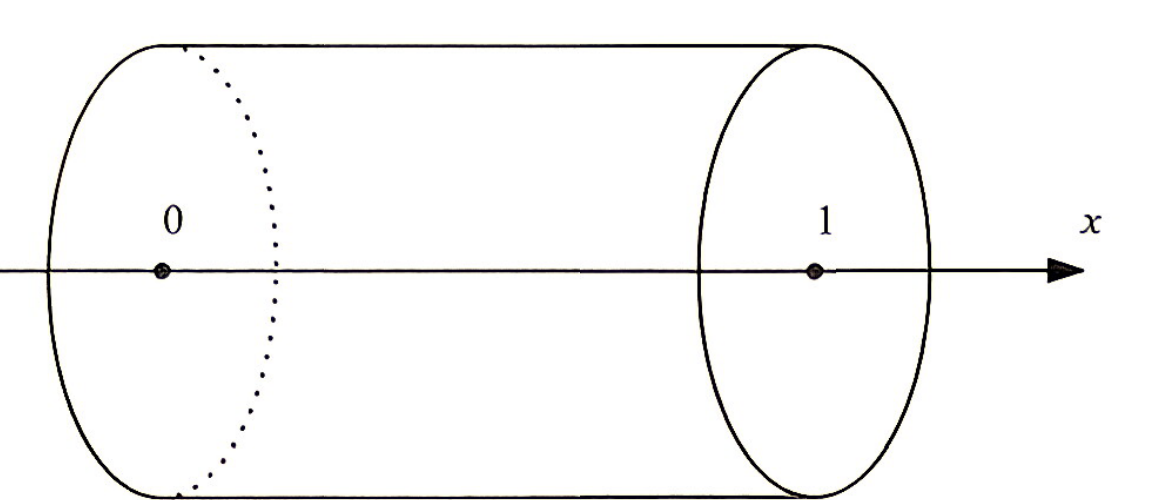
\includegraphics[width=0.62\linewidth]{figures/fig_p056_1.png}
  \caption*{图 2.6\quad 标准柱面 $C_{\mathrm{cyl}}$（原书 p.48, Figure 2.6；PDF p.56）}
\end{figure}
\[
  H(x,\theta,p_x,p_\theta)=\frac12\big(p_x^2+p_\theta^2\big),
\]
其中 $(x,\theta,p_x,p_\theta)\in T^*\R^2$，而 $p_x$ 与 $p_\theta$ 表示余向量。

哈密顿系统 $(T^*\R^2,\omega_{\mathrm{can}},H)$ 事实上是完全可积的（这里只需再找一个
满足定义 2.6.1 中条件的哈密顿函数 $H_2$）。为验证这一点，把 (2.6) 中的哈密顿方程
应用于当前设定，得到如下方程组
\begin{equation}
  \dot x=p_x,\qquad \dot\theta=p_\theta,\qquad
  \dot p_x=0,\qquad \dot p_\theta=0 .
  \tag{2.36}
\end{equation}
令 $H_2:=p_\theta$，则
\[
  \{H,H_2\}=\{H,p_\theta\}=-\{p_\theta,H\}
  =-\dd p_\theta(X_H)=0,
\]
其中最后一个等号来自 (2.36) 中的第四个方程。此外，只要 $p_x\neq0$，$\dd H$ 与
$\dd H_2$ 就线性无关。由于 $p_x$ 是 $T^*\R^2$ 上的连续函数，$\{p_x=0\}$ 的补集
当然是开稠密子集。
% [Tutor Note: 此处 $\{-,- \}$ 与 $\dd p_\theta(X_H)$ 的换算直接来自定义 2.3.1：
% $\{p_\theta,H\}=\dd p_\theta(X_H)$，而 $\{H,p_\theta\}=-\{p_\theta,H\}$ 由斜对称性
% (2.9) 得到；$X_H$ 的 $p_\theta$ 分量为 $\dot p_\theta=0$，故 $\dd p_\theta(X_H)=0$。
% 另注意 $T^*\R^2$ 与 $T^*\T^2$ 在 $x$ 方向周期化后等同，故下文同时使用两种写法。]

现在我们有几点初等的观察。

(i) 取 $\Big(\dfrac12,0\Big)\in\R^2$，则 $(H,H_2)$ 的原像为
\begin{align*}
  (H,p_\theta)^{-1}\Big(\frac12,0\Big)
  &=\big\{(x,\theta,p_x,p_\theta)\in T^*\R^2\bigm|\,p_x^2+p_\theta^2=1
    \ \text{且}\ p_\theta=0\big\}\\
  &=\big\{(x,\theta,\pm1,0)\bigm|x,\theta\in S^1\big\}
  =\T^2\sqcup\T^2 .
\end{align*}
此外，每个 $\T^2$ 都是拉格朗日的，且哈密顿动力学保持在其中——即每条从某个 $\T^2$ 出发
的哈密顿轨道都留在该 $\T^2$ 内。因此，$\T^2$ 有时被称为\emph{不变环面}。

(ii) $(H,p_\theta)^{-1}\Big(\dfrac12,0\Big)$ 中的每个 $\T^2$ 都有邻域
$\nu(\T^2)\subset T^*\R^2$（或 $T^*\T^2$ 中的邻域），它可如下分裂
\begin{equation}
  \nu(\T^2)\cong\T^2\times\mathbb{D}^2 .
  \tag{2.37}
\end{equation}
% >>> p057
这里 $\mathbb{D}^2=\mathbb{D}^2(p_x,p_\theta)$ 是点 $(p_x,p_\theta)=(1,0)$ 或 $(-1,0)$ 附近的小圆盘状
邻域。例如，不取上面 (i) 中的单个点，而考虑矩形
\[
  \Big(\frac12-\epsilon,\frac12+\epsilon\Big)\times(-\epsilon,\epsilon)\subset\R^2 .
\]
则它在 $(H,p_\theta)$ 下的原像是以 $(1,0)$ 或 $(-1,0)$ 邻域中的 $(p_x,p_\theta)$ 为参数
的一族 $\T^2$。这样，相对于 (2.37) 的分裂，$\nu(\T^2)$（平凡地）具有坐标，形式为：
$\T^2$ 上的 $\varphi:=(x,\theta)$ 与 $\mathbb{D}^2$ 上的 $S:=(p_x,p_\theta)$。由 $T^*\R^2$ 上
的标准辛结构 $\omega_{\mathrm{can}}$（或其诱导到 $T^*\T^2$ 上的辛结构）可知，相对于
此辛结构，$\T^2$ 与 $\mathbb{D}^2$ 都是拉格朗日的。

(iii) 在上面 (ii) 引入的坐标 $(\varphi,S)$ 下，$H$ 与 $p_\theta$ 的哈密顿流在
$\nu(\T^2)$ 内是线性的。确切地说，二者都具有如下形式
\begin{equation}
  (\varphi,S)\mapsto(\varphi+tq(S),S),
  \tag{2.38}
\end{equation}
其中 $q(S)$ 是 $S$ 的函数。事实上，对由 $H$ 生成的哈密顿流的某条闭轨道
$\{x(t),\theta(t),p_x(t),p_\theta(t)\}_t$，由哈密顿方程 (2.36) 及初值
$(x_0,\theta_0,(p_x)_0,(p_\theta)_0)$，由 (2.36) 的第三、第四式得
$p_x(t)=(p_x)_0$、$p_\theta(t)=(p_\theta)_0$，从而
\[
  x(t)=x_0+t(p_x)_0\qquad\text{以及}\qquad
  \theta(t)=\theta_0+t(p_\theta)_0 .
\]
再译成 (2.38)，便有 $q(S)=q(p_x,p_\theta)=(p_x,p_\theta)$，即恒等映射。对哈密顿函数
$p_\theta$ 有类似的论证。\hfill$//$
\end{wexam}
% [Tutor Note: 本例中 $q$ 之所以恰为恒等映射，是因为 $H=\frac12(p_x^2+p_\theta^2)$ 的
% 哈密顿流在 $(x,\theta)$ 上就是平移 $(x,\theta)\mapsto(x+tp_x,\theta+tp_\theta)$；
% 一般可积系统中 $q(S)$ 是非线性的（即频率 $\partial H/\partial S$ 随作用量变化）。
% 另外，$p_x=\pm1$ 对应原像分裂成两个连通分支 $\T^2\sqcup\T^2$，这正是
% $(s,t)=(1/2,0)$ 是正则值却有两个原像分支的原因；在同调意义下这两支分别对应
% 不同的「能量面」。]

下面的练习鼓励有兴趣的读者处理一个颇为类似的情形，同样是在例 2.8.1 那样的旋转曲面上，
只是轮廓函数略有不同。

\begin{wexer}{2.8.1}
（参见 [211] 的附录）对 $\R^3$ 中轮廓函数 $f(x)$ 由图 2.7 给出的旋转曲面，验证例 2.8.1
中的观察 (i)、(ii)、(iii)。这里旋转轴为 $x$-轴，$f(x)$ 定义在区间 $[0,1]$ 上，在
$x=0.5$ 处恰有一个极大值点，且关于 $x=0.5$ 对称。此外，这里假设 $|f(x)|_{C^0}$ 很小，
如图 2.7 所示 $f(0.5)=3\epsilon$，其中 $\epsilon>0$ 很小。
\end{wexer}

\begin{figure}[htbp]
  \centering
  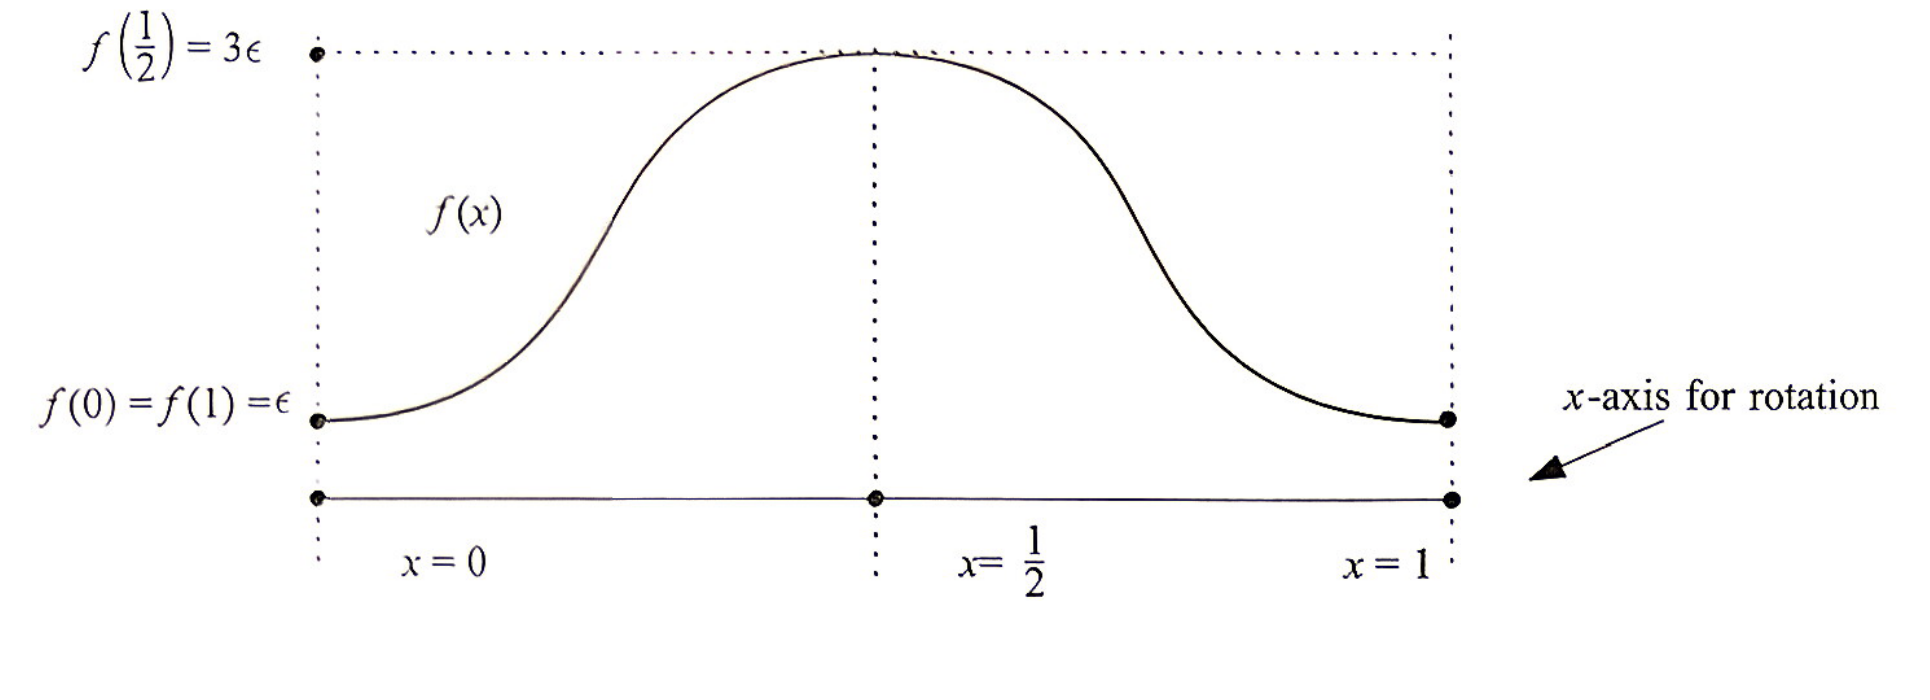
\includegraphics[width=0.88\linewidth]{figures/fig_p058_1.png}
  \caption*{图 2.7\quad 旋转曲面的轮廓函数 $f(x)$（原书 p.50, Figure 2.7；PDF p.58）}
\end{figure}

无论得自本节开头的讨论，还是得自例 2.8.1（或练习 2.8.1）中的观察，我们所发现的这一
现象都是如下著名结果的特例，该结果保证任意可积系统局部上具有简单的结构。

% >>> p058
\begin{wthm}{2.8.1}
（Arnold--Liouville 定理，见 [15] 第 10 章第 49.A 节）给定（完全）可积系统
$(M^{2n},\omega,H)$，其中 $\{H_i\}_{i=1}^n$ 是定义它的 Poisson 交换哈密顿函数组，则
我们有如下局部描述。
\begin{enumerate}[label=(\roman*)]
  \item 对 $F:=(H_1,\cdots,H_n)$ 的任意正则点 $p$，若 $p$ 的原像是紧的，则
        $L:=F^{-1}(p)$ 是 $(M,\omega)$ 中的一个拉格朗日环面。
  \item 上面 (i) 中的环面 $L$ 在 $M$ 中有邻域 $\nu(L)$，使得在微分同胚意义下
        $\nu(L)$ 分裂为 $\T^n\times\mathbb{D}^n$，即环面 $\T^n$ 上以圆盘状纤维构成的平凡丛。
        此外，$\nu(L)$ 具有坐标系（称为\textbf{作用量–角坐标}，action-angle coordinate），
        记作 $(\varphi,S)=(\varphi_1,\cdots,\varphi_n,S_1,\cdots,S_n)$，其中 $\varphi$
        定义在 $\T^n$ 分量上（称为\emph{角}），$S$ 定义在 $\mathbb{D}^n$ 分量上（称为\emph{作用量}），
        使得在辛同胚意义下辛结构 $\omega$ 可表示为 $\sum_i\dd S_i\wedge\dd\varphi_i$。
  \item 在邻域 $\nu(L)$ 中，在 (ii) 引入的坐标 $(\varphi,S)$ 下，每个 $H_i$ 的哈密顿流
        是线性的，即它可表示为 $(\varphi+tq(S),S)$，其中 $q=q(S)$ 为某函数。
\end{enumerate}
\end{wthm}
% [Tutor Note: (ii) 中的表达式 $\omega=\sum_i\dd S_i\wedge\dd\varphi_i$ 与本书
% $\omega_{\mathrm{can}}=\sum_i\dd p_i\wedge\dd q_i$ 的约定一致（$S$ 对应动量、$\varphi$
% 对应位置）。作用量 $S$ 的一个内蕴刻画是 $S_i=\frac{1}{2\pi}\int_{\gamma_i}\lambda$，
% 其中 $\lambda$ 是 $\omega=-\dd\lambda$ 的局部原形式、$\gamma_i$ 是环面上第 $i$ 个
% 基本闭链；这解释了「作用量」一名。定理要求 $L$ 紧（否则只得到
% $\R^{n-k}\times\T^k$，见注 2.8.2），并要求 $F$ 的流是完备的（"complete"）。
% 术语依据：action-angle coordinate 通行译作「作用量–角坐标」。]

对该定理最早已知的证明，见 [159,160]。

\begin{wrem}{2.8.1}
由定义 2.5.2，紧 $2n$ 维辛环面流形 $(M,\omega)$ 具有矩映射 $\mu:M\to\R^n$；由例 2.6.3
知，这样的 $(M,\omega,H)$ 总是可积的，其中 $H$ 为 $\mu$ 的任一分量（看作 $M$ 上的
哈密顿函数）。于是定理 2.8.1 表明，任何辛环面流形本质上都被拉格朗日环面叶状化，这些
环面大多是矩像中正则值在 $\mu$ 下的原像。若 $(M,\omega)$ 具有非空边界，上述结论对其
内部成立（在边界上可能出现某种退化）。
\end{wrem}

这里我们不会给出定理 2.8.1 的完整证明（完整证明见 [30] 第 1.4 节）。作为替代，我们将
在
% >>> p059
$4$ 维情形下重新表述定理 2.8.1 的结论 (i) 并概述其证明。当我们将在第 9 章系统地研究
拉格朗日子流形时，这一结果会特别有用。

\begin{wprop}{2.8.1}
给定辛流形 $(M^4,\omega)$ 与两个函数 $H,G:M\to\R$，使得它们 Poisson 交换，即
$\{H,G\}=0$。则对函数 $(H,G):M\to\R^2$ 的任意正则值 $(s,t)\in\R^2$，若其原像
$(H,G)^{-1}(s,t)$ 连通且紧，则它是 $(M^4,\omega)$ 中的一个拉格朗日环面。
\end{wprop}

\begin{wproof}
考虑如下定义的 $\R^2$ 在 $M$ 上的作用：对任意 $(a,b)\in\R^2$ 与点 $x\in M$，考虑映射
\begin{equation}
  (a,b)\cdot x:=\varphi_{X_G}^b\circ\varphi_{X_H}^a(x).
  \tag{2.39}
\end{equation}
对 $L:=(H,G)^{-1}(s,t)$，由于 $(s,t)$ 是正则值，$L$ 是 $M$ 中的 2 维子流形。注意 $L$
也可写成 $L=H^{-1}(s)\cap G^{-1}(t)$，于是 $\R^2$ 在 $M$ 上的作用限制为 $L$ 上的作用，
因为哈密顿流 $\varphi_{X_H}^a$ 保持 $H$ 的水平集（因 $\{H,H\}=0$），同时也保持 $G$ 的
水平集（因 $\{H,G\}=0$）。由于假定 $L$ 连通，这一作用使我们能把 $L$ 写成单个轨道空间，
即对任意点 $p\in L$ 有
\[
  L=\R^2\cdot\{p\}\cong\R^2/(\R^2)_p,
\]
其中 $(\R^2)_p$ 表示该作用在点 $p$ 处的稳定化子。注意 $(\R^2)_p$ 是 $\R^2$ 中的秩 2
格（lattice）（因为它离散，且 $L$ 假定紧），由此得出 $L$ 在拓扑上是一个环面。此外，
在每一点 $p\in L$，其切空间 $T_pL$ 具有基，基元为 $X_H(p)$ 与 $X_G(p)$。于是
\[
  \omega_p(X_H(p),X_G(p))=\{G,H\}(p)=\{H,G\}(p)=0 .
\]
因此，$L$ 是拉格朗日环面。
\end{wproof}
% [Tutor Note: 证明的关键在于 (2.39) 确实定义 $\R^2$ 的作用：由 (2.10) 与
% $\{H,G\}=0$ 得 $[X_H,X_G]=X_{\{H,G\}}=0$，故两个哈密顿流可交换，
% $(a,b)\mapsto\varphi^b_{X_G}\circ\varphi^a_{X_H}$ 是群同态（这里 $\varphi^t_X$ 记
% 向量场 $X$ 的时间 $t$ 流）。$\{H,H\}=0$ 是自动成立的三 (iii) 条；两处用到 $\{H,G\}=0$：
% 一处保证作用良定义在水平集上，一处保证 $X_H,X_G$ 张成迷向平面。稳定化子离散且
% $L\cong\R^2/\Gamma$ 紧，故 $\Gamma$ 是秩 2 格，$L\cong\T^2$。]

回顾命题 2.8.1 的证明，假设 $\{H,G\}=0$ 用在两处：一是确认作用 (2.39) 在
$L=(H,G)^{-1}(s,t)$ 上良定义；二是构成 $L$ 的切空间的一组拉格朗日基。

\begin{wrem}{2.8.2}
命题 2.8.1 的同一结论对任意 $(M^{2n},\omega)$ 与 $n$ 个 Poisson 交换的哈密顿函数
成立，且在同样假设下原像将是 $n$ 维拉格朗日环面。若去掉 $L$ 紧的假设，同样的论证
依然成立，唯一的差别是原像 $(H,G)^{-1}(s,t)$ 将具有 $\R^{n-k}\times\T^k$ 的形式，
可能非紧。
\end{wrem}
% [Tutor Note: 注 2.8.2 中的 $\R^{n-k}\times\T^k$ 来自稳定化子 $(\R^n)_p$ 的秩 $k$：
% 若水平集紧，则 $\Gamma=(\R^n)_p$ 是秩 $n$ 的格，得 $\T^n$；不再紧时秩 $k$ 可以小于
% $n$，剩余的 $n-k$ 个方向给出非紧的 $\R^{n-k}$ 因子。这里 $k=0$ 时对应完全非紧的
% $\R^n$ 纤维，$k=n$ 时回到环面。]
